\section{Results}
\label{sec:results}

\subsection{From Negative $R^2$ to Economic Evaluation}

The early model comparison gave a clear warning sign: raw ETF expansion was not a robust way to improve daily stock-return prediction. Out-of-sample $R^2$ was generally negative, and the raw ETF model underperformed due to dimensionality and noise. This negative result is important because it motivates the later design choice: compress ETF information and evaluate it economically rather than relying on statistical fit alone.

\subsection{Initial Four-Model Comparison}

The first clean lesson comes from the initial four-model comparison: baseline, baseline+ETF, baseline+network, and baseline+ETF+network. Table~\ref{tab:initial-models} reports the gross AlphaMark Sharpe ratios at the full-universe slice (\texttt{qr\_100}).

\begin{table}[H]
\centering
\caption{Initial four-model comparison using gross AlphaMark Sharpe at \texttt{qr\_100}.}
\label{tab:initial-models}
\begin{tabular}{lcc}
\toprule
Model & cap250k & mktcap \\
\midrule
Baseline HAR & 0.604 & 0.657 \\
Baseline + raw ETF block & 0.311 & 0.099 \\
Baseline + network & -0.094 & -0.052 \\
Baseline + ETF + network & 0.087 & -0.020 \\
\bottomrule
\end{tabular}
\end{table}

This table and Figure~\ref{fig:initial-models} capture the central empirical tension in the project. The baseline is strong. The raw ETF block does not improve on it and often performs much worse. The network-style extension is conceptually interesting, but in this implementation it does not survive as a competitive gross strategy. These early results indicate that the incremental content in ETF-linked variables is limited when used directly and requires a narrower specification.

\begin{figure}[H]
\centering
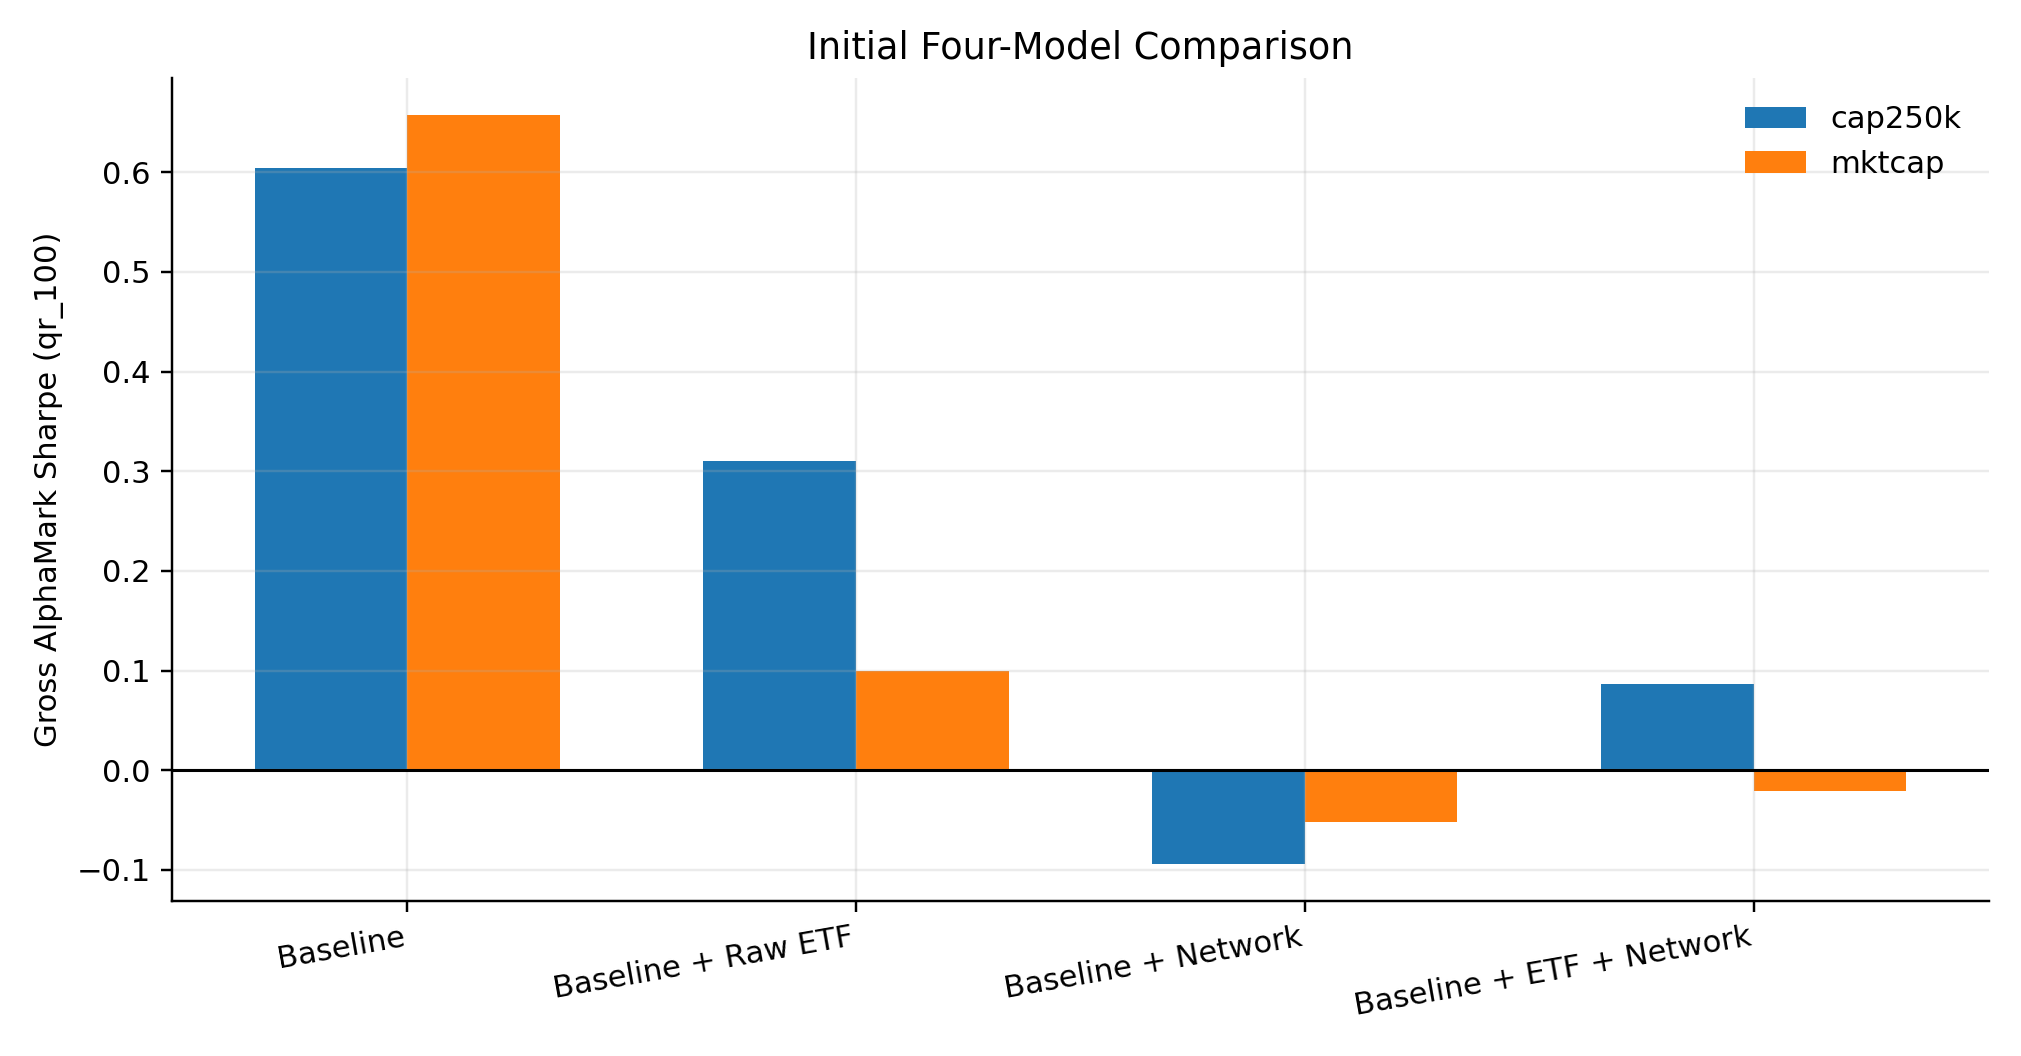
\includegraphics[width=0.92\linewidth]{figures/initial_model_comparison.png}
\caption{Gross AlphaMark Sharpe for the initial four-model comparison at \texttt{qr\_100}. The main empirical message is that the stock-only baseline is strong, raw ETF expansion is much weaker, and the pure network-style extension does not become competitive in this implementation.}
\label{fig:initial-models}
\end{figure}

\subsection{Cost-Adjusted Ranking of Final Strategies}

Table~\ref{tab:final-strategies} summarizes the three final strategies. The strongest 20 bps net result is the consensus-majority ETF strategy, while the regime strategy is the most resilient at higher cost levels. The baseline remains a strong benchmark once it is evaluated under comparable execution constraints, so the appropriate interpretation is not ``ETF beats baseline everywhere.'' Rather, ETF-conditioned strategies become competitive and in some settings superior once the trading rule is specified carefully.

\begin{table}[H]
\centering
\caption{Summary of the final low-turnover strategies. Gross AlphaMark Sharpe is shown using the strongest quantile slice from the updated multi-quantile AlphaMark reports. Net Sharpe numbers come from the separate turnover-based cost review.}
\label{tab:final-strategies}
\begin{tabular}{lcccc}
\toprule
Strategy & Best gross Sharpe & Net 10 bps & Net 20 bps & Net 50 bps \\
\midrule
Consensus majority ETF & 0.558 & 0.482 & 0.417 & 0.221 \\
Blend top3 & 0.598 & 0.419 & 0.373 & 0.259 \\
Regime & 0.525 & 0.452 & 0.404 & 0.279 \\
Optimized baseline benchmark & 0.657 & 0.500 & 0.373 & 0.259 \\
\bottomrule
\end{tabular}
\end{table}

The ranking across cost regimes is informative, as summarized in Figure~\ref{fig:cost-robustness}. At 10 bps, the optimized baseline remains extremely strong. At 20 bps, the consensus-majority ETF strategy becomes the strongest of the final three and slightly exceeds the optimized baseline benchmark. At 50 bps, the regime strategy becomes relatively more robust. This pattern is consistent with ETF-linked information being most useful when it helps screen marginal trades rather than when it is used to support frequent repositioning.

Appendix~\ref{sec:appendix-impl} records the exact rolling-window design and the representative implementation parameters used in the central 20 bps comparison.

\begin{figure}[H]
\centering
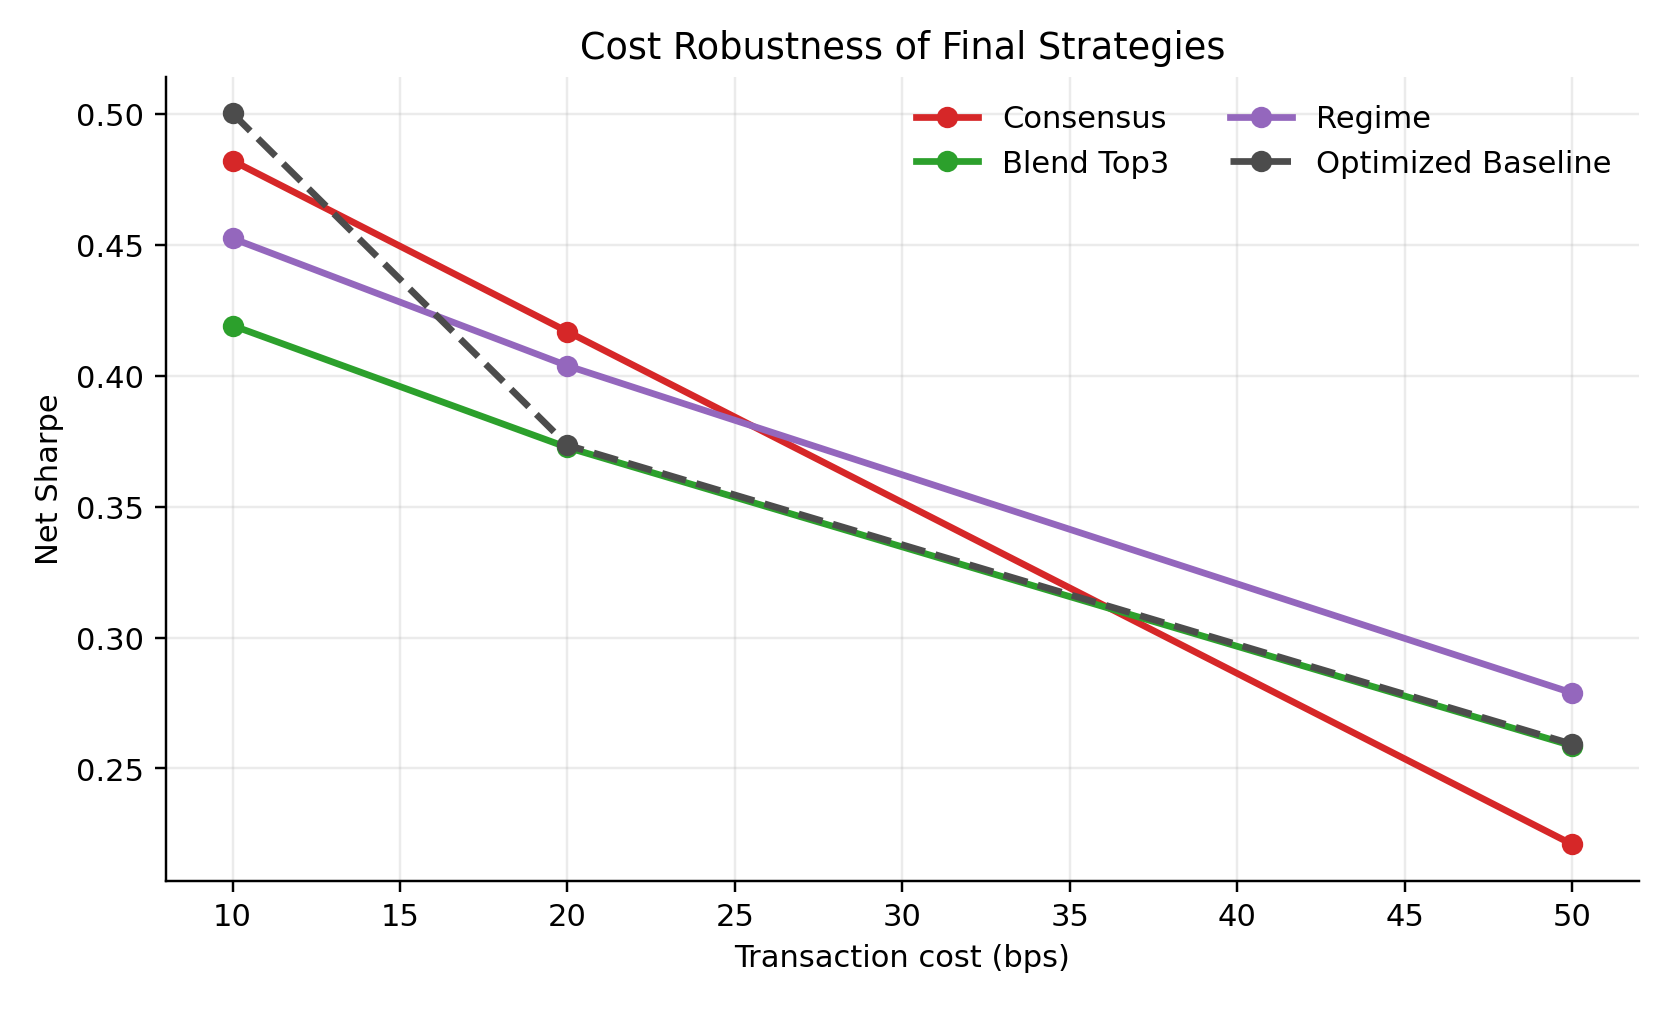
\includegraphics[width=0.84\linewidth]{figures/cost_robustness.png}
\caption{Net Sharpe under 10, 20, and 50 bps cost assumptions. The optimized baseline remains a strong benchmark, but the ETF-conditioned strategies become competitive once execution is slowed down, with consensus strongest around 20 bps and regime most resilient at 50 bps.}
\label{fig:cost-robustness}
\end{figure}

Figure~\ref{fig:net-paths} plots the cumulative net return paths for the central 20 bps case. This is the cleanest like-for-like comparison because it uses each strategy's representative implementation under the same cost assumption. The figure shows that the ETF-conditioned strategies are not merely producing isolated high-Sharpe summaries; they also generate sustained cumulative performance paths that are comparable to, and in some periods stronger than, the optimized baseline.

\begin{figure}[H]
\centering
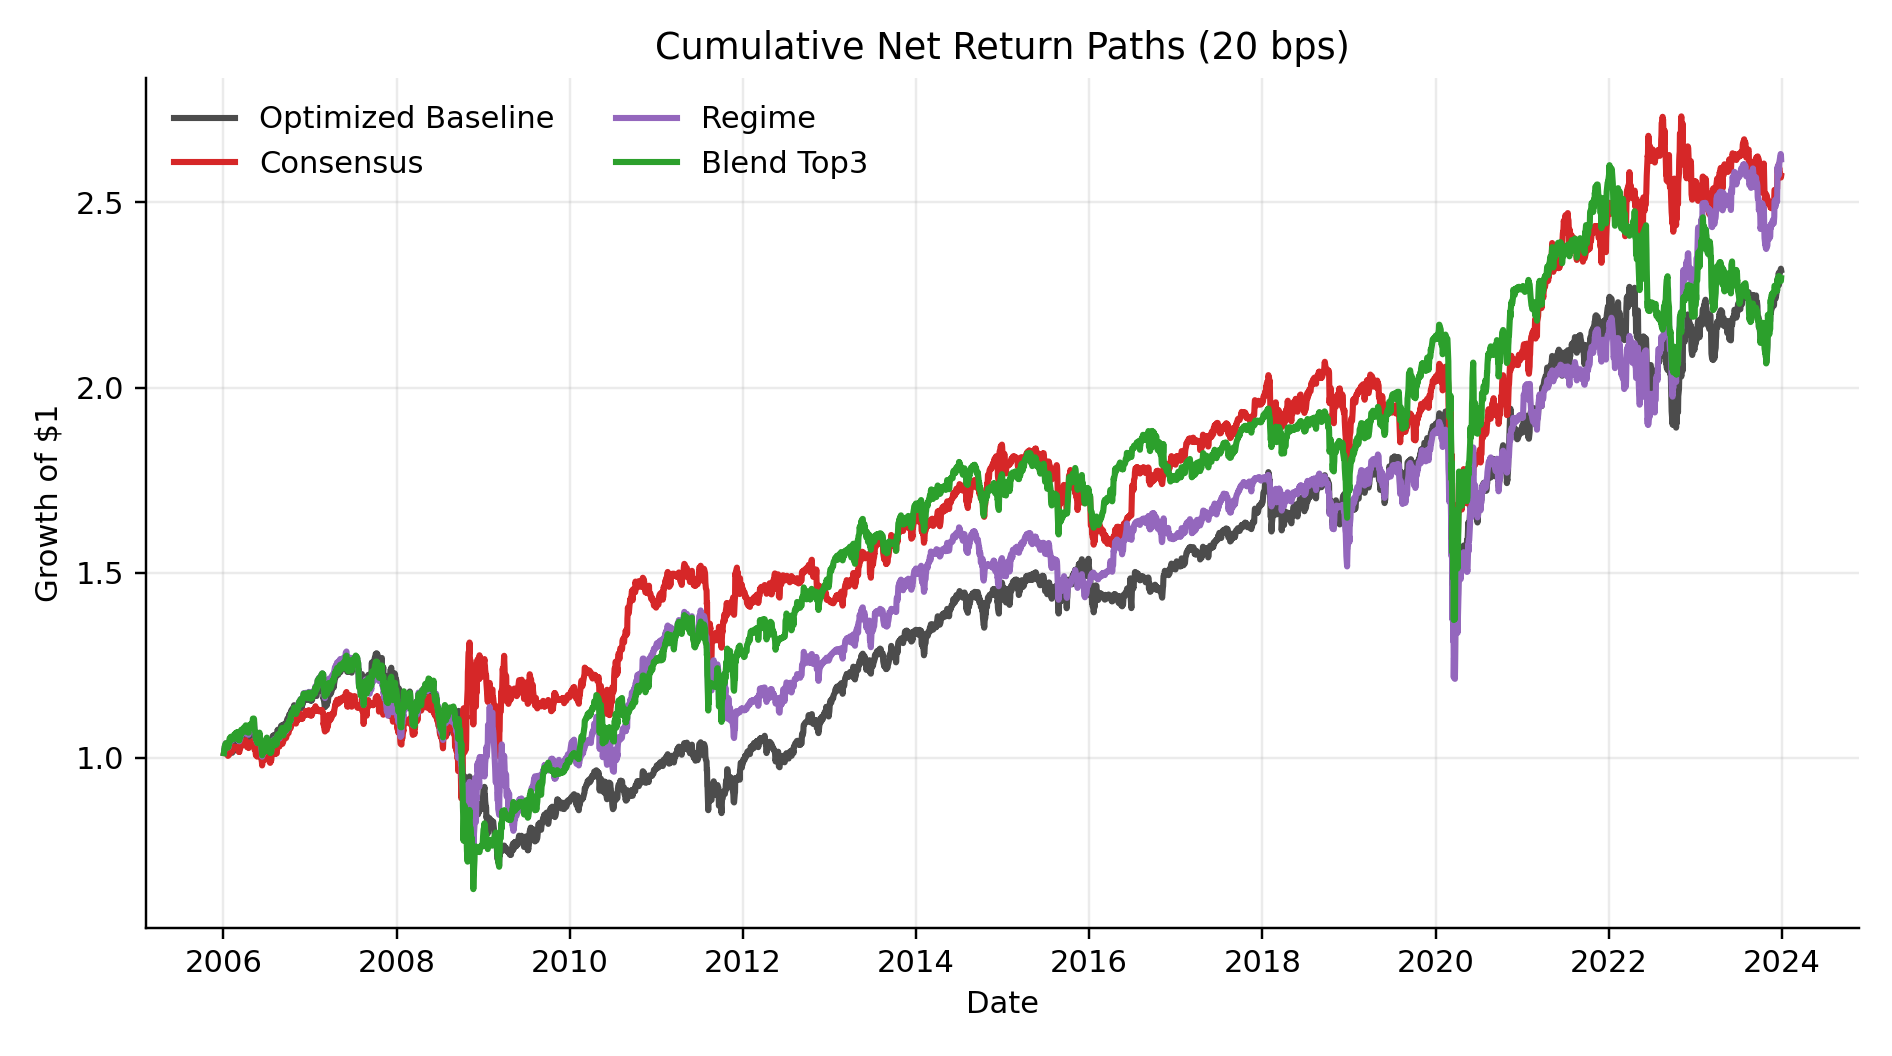
\includegraphics[width=0.88\linewidth]{figures/net_cumulative_paths_20bps.png}
\caption{Cumulative net return paths at 20 bps for the optimized low-turnover baseline and the three final ETF-conditioned strategies. This central-cost comparison makes the economic significance of the strategies visually transparent and highlights that the final strategies should be viewed as competitive refinements to a strong baseline benchmark.}
\label{fig:net-paths}
\end{figure}

\subsection{AlphaMark Quantile Results}

The updated AlphaMark reports now include \texttt{qr\_100}, \texttt{qr\_75}, \texttt{qr\_50}, and \texttt{qr\_25}. This matters because the best slices do not always occur at the full-universe level. For example, the strongest gross AlphaMark Sharpe for the consensus strategy occurs at \texttt{qr\_75} with market-cap sizing (about 0.558), while the strongest gross slice for the blend and regime strategies appears around \texttt{qr\_50} with equal-weight sizing (about 0.598 and 0.525, respectively).

This quantile evidence, visualized in Figure~\ref{fig:qmulti}, supports the general interpretation that the signals contain useful cross-sectional ranking information even when the full-universe portfolio is not always the best-performing gross configuration. Put differently, ETF-conditioned signals do not merely alter average portfolio exposure; they also help reshape the cross-sectional ordering of names.

\begin{figure}[H]
\centering
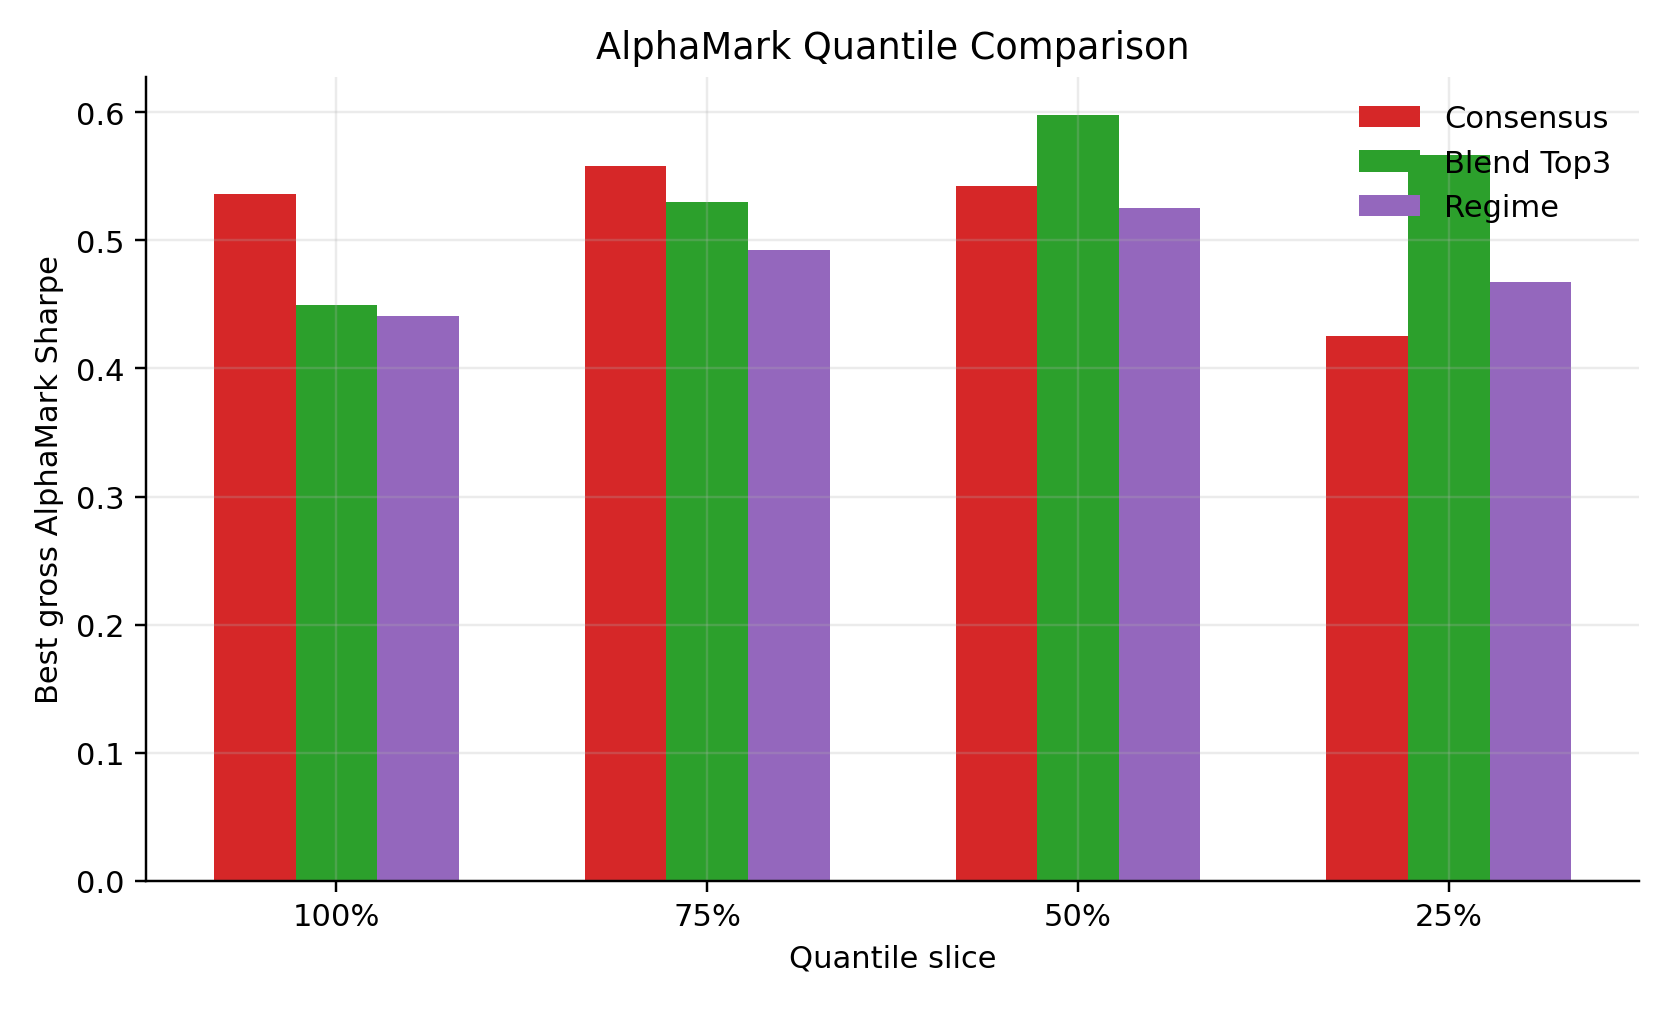
\includegraphics[width=0.84\linewidth]{figures/alphamark_quantile_comparison.png}
\caption{Best gross AlphaMark Sharpe by quantile slice for the three final strategies. The strongest slice is not always the full-universe portfolio, which suggests that the ETF-conditioned signals contain useful cross-sectional ranking information.}
\label{fig:qmulti}
\end{figure}

\subsection{Liquidity Diagnostic}

We also ran a normalized-dollar-volume bucket analysis. The main result is not that one specific liquidity bucket drives all performance. In fact, when the strategy is restricted to a single bucket, net Sharpe typically worsens. However, on a gross basis, the ETF-conditioned strategies look cleaner in the middle-to-upper liquidity buckets than in the extreme low- or high-activity buckets. For instance, the consensus strategy is strongest in the middle buckets on a gross basis, whereas single-bucket net performance remains poor across the board.

This suggests that ETF-linked information may be more reliable in moderate liquidity states, but that the final alpha still needs broad cross-sectional diversification to survive costs. In other words, normalized liquidity is a useful diagnostic variable, but not a sufficient standalone trading filter. Figure~\ref{fig:liquidity} is therefore best read as an implementation diagnostic rather than as an argument for a single-bucket trading rule.

\begin{figure}[H]
\centering
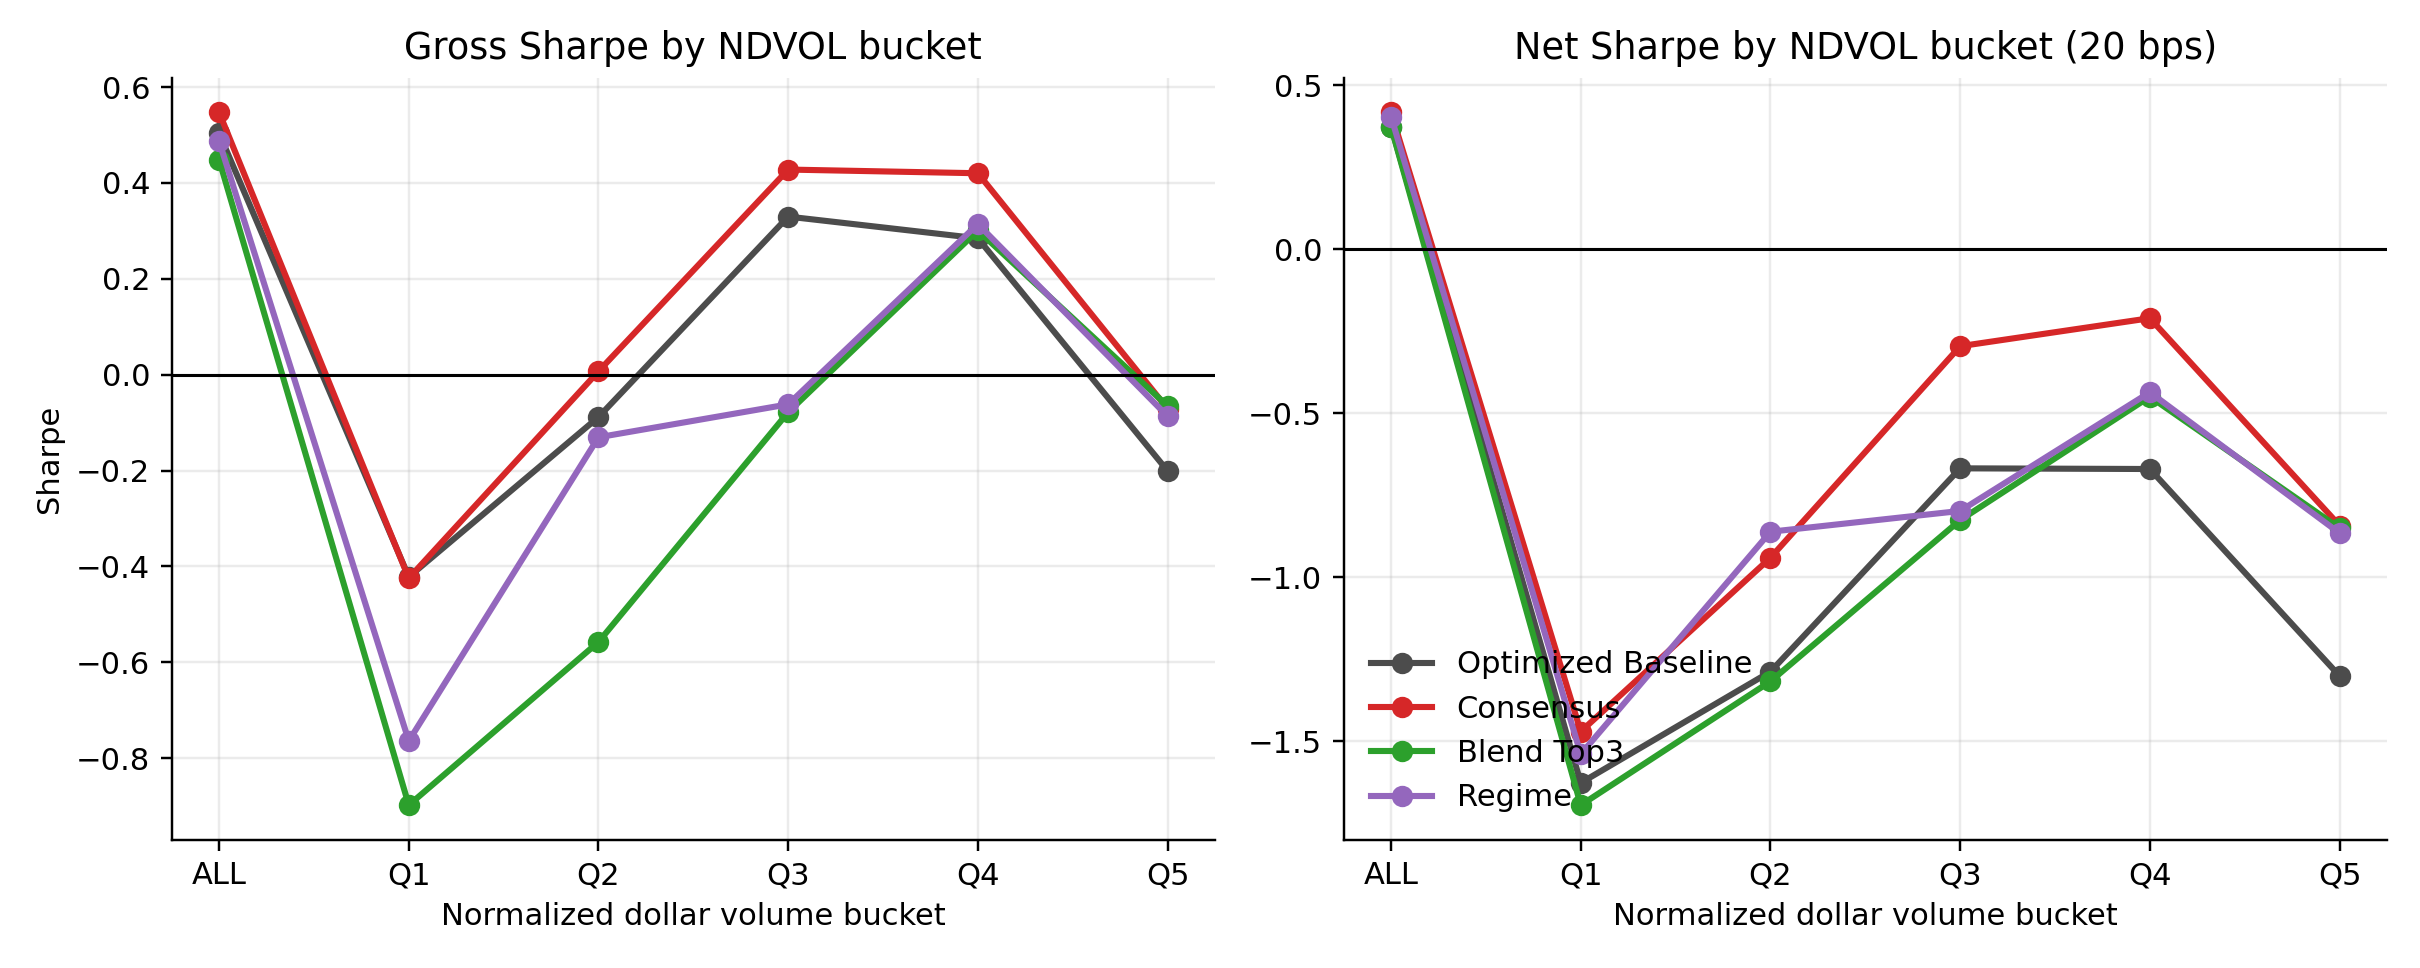
\includegraphics[width=\linewidth]{figures/liquidity_bucket_diagnostic.png}
\caption{Liquidity-state diagnostic based on normalized dollar volume (NDVOL). On a gross basis, the ETF-conditioned strategies look cleaner in the middle buckets. On a net basis, restricting the strategy to a single bucket worsens performance, which suggests that broad cross-sectional diversification remains important.}
\label{fig:liquidity}
\end{figure}
